\chapter{Procedural Content Generation (PCG) Background}
\label{ch:backgroundpcg}
The generation of procedural content is important for many real-time applications. 
The main use for PCG in the past has been the generation of content which is too labour intensive for artists to create by hand.
Examples of this will be seen in Section~\ref{sec:citygen} where whole cities are generated using PCG.
Other research has been done on the generation of building interiors as described in Section~\ref{sec:buildinginteriors}.
We also see how realistic looking materials can be generated using techniques such as Perlin Noise in Section~\ref{sec:perlinnoise} and with bump mapping effects in Section~\ref{sec:bumpmapping}.

Overall it is hoped that this chapter can convey that PCG includes a wide variety of techniques, but we will generalise them into two categories:
\begin{itemize}
	\item Geometry Generation
	\item Texture Generation
\end{itemize}
Using this general classification as a guide, the design of the system presented in Chapter \ref{ch:design} will use some of the techniques presented here to create the prototype game application.

\section{Geometry Generation}
\subsection{City Generation}
\label{sec:citygen}
Recently, there has been much interest in the procedural generation of cities.
Ma\"{i}m et al.~\cite{maim2007populating} demonstrated how it is possible to recreate the population of historic cities using procedural techniques.
The use of procedural techniques to generate the crowds in Pompeii allowed realtime simulation with great variety in character representation.
This would not have been possible with traditional modelling techniques.

The Metropolis project~\cite{web:metropolis} investigates the simulation of crowds in a modern city context.
Members of the crowd are modelled based on a variation of some template.
Different clothes are applied to the same templates to give the illusion of variation in the character models~\cite{mcdonnell2007pipeline}.
People are represented as agents which react to their environment~\cite{ulicny2002towards}.
In this way crowds are simulated using a variety of procedural techniques.

\begin{figure}
  \centering
    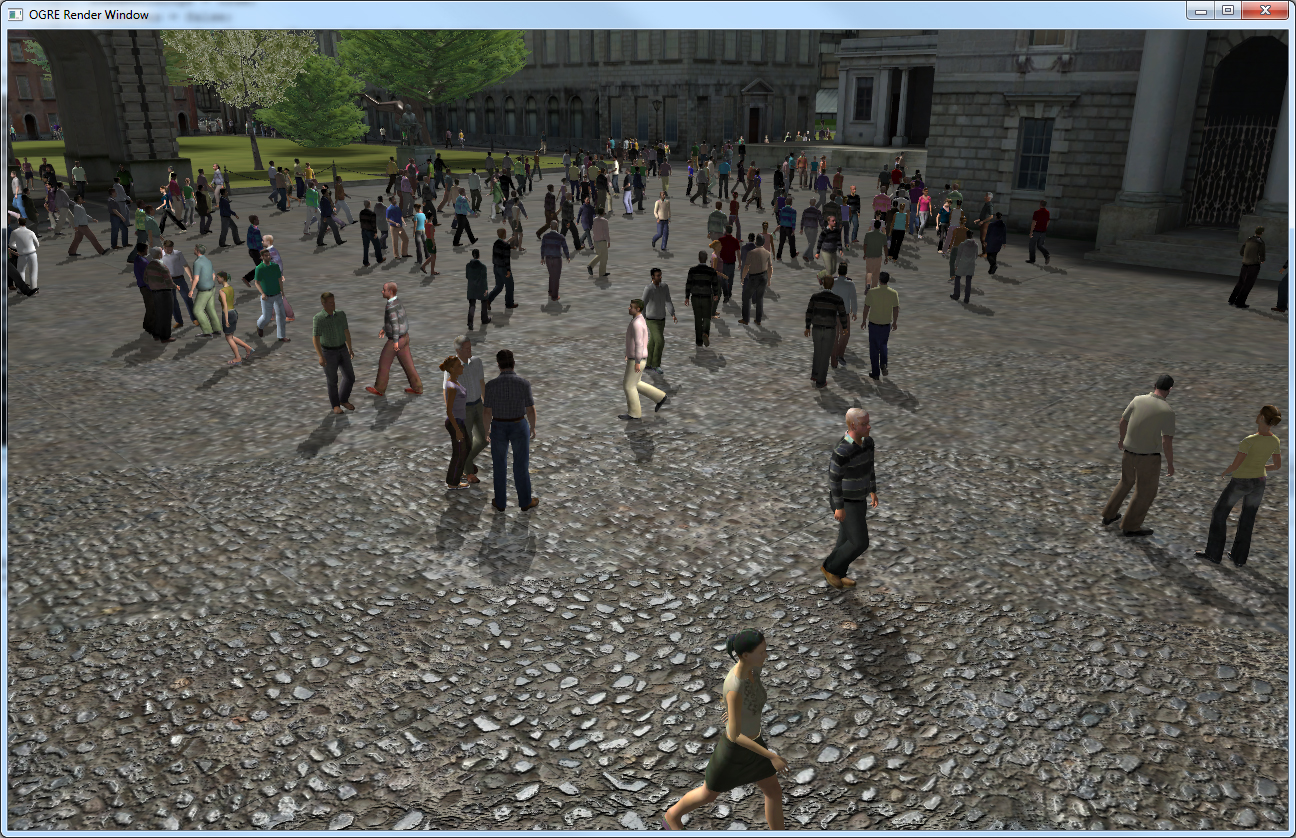
\includegraphics[width=0.7\textwidth]{images/metropolis}
  \caption{Screenshot of the Metropolis program in action}
\end{figure}

CityEngine by Parish et. al is an example of how procedural techniques can be applied to generates environments of great depth~\cite{parish2001procedural}.
Using a combination of extended L-systems and self-sensitive L-systems, roads are generated which realistic simulate that of a target city.
Plans of buildings are generated between road segments in a recursive subdivision scheme, which discards inaccessible buildings.
The models of buildings are generated using an L-system using the bounding box of the building as the axiom of the L-system.
A technique known as \emph{layered grids} is proposed for the procedural generation of interesting textures for buildings.

\begin{figure}
  \centering
    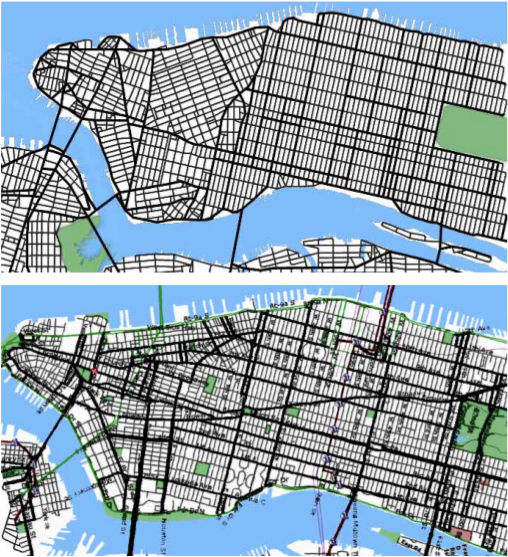
\includegraphics[width=0.7\textwidth]{images/cityengine}
  \caption{Above: Street plan generated by CityEngine. Below: Actual plan of central manhattan.}
\end{figure}

Wonka et. al present a method for automatically modelling architecture which generates a wide range of architectural features~\cite{wonka2003instant}.
A new type of design grammar known as a ``Split grammars'' is used to derive building designs.
This allows the restriction of types of allowed rules. 
These restrictions make the grammars powerful enough for the modelling of buildings.
A parameter matching system allow the user to specify multiple high-level design goals so that the output appears consistent.
Control grammars are introduced which are simple context free grammars which handle spatial ideas in an orderly way which corresponds to architectural principles.
This paper's method gives a useful insight into how architectural features may be used to further enhance the generation of buildings in a procedural way.
We will see in the design of the system we present in Chapter~\ref{ch:design}, how different types of plans can be generated using a small number of input parameters.

\subsection{Building Interiors}
\label{sec:buildinginteriors}
CityEngine provides a method for generating the exteriors of buildings, however this project will focus on the generation of indoor environments using procedural techniques.
Greuter et al. provide methods for generating floor plans of buildings in a procedural fashion~\cite{greuter2003real}.
Plans are generated by merging various polygonal shapes in a pseudo-random fashion to generate a final plan of a series of floors.
These floor plans are extruded into the 3rd axes and the outdoor building models are created from this.
The floors are not populated with rooms however as the indoor environments are not meant to be seen.

So et al. use wall extrusion for generating 3D indoor environments from floor plans~\cite{so1998reconstruction}.
These generated indoor environments contain rooms.
So et al. apply the technique to a CAD tool, but the technique could easily be applied to an OpenGL-based environment also.
Using So et al.'s work as a guide, the plan extrusion techniques presented in Section~\ref{sec:planextr} were developed.

Hahn et al present a novel approach to the generation of virtual building interiors in real-time~\cite{hahn2006persistent}.
The approach uses a lazy generation scheme which is advantageous as it means that the amount of memory used is small. 
They divide the interiors of buildings into temporary regions and built regions.
Built regions contain the final visible product of the generator and hold the geometry needed for collision detection and rendering.
Temporary regions are placeholder regions which are turned into built regions in a lazy fashion.
Temporary regions are populated when the player enters them, via a portal system.
The generation of built regions is split into stages to simplify the implementation:
\begin{enumerate}
	\item Building Setup : Anything which effects multiple floors is generated at this stage. Elevators and stairs are included as well as global textures.
	\item Floor Division : Divides the building into evenly spaced floors. Floors are then divided into 2 parts.
	\item Hallway Division : Hallways are constructed by dividing the regions around other blocks which can be rectangular loops or straight segments of hallway. 
	\item Room Cluster Division : Regions between hallways are divided into rooms. 
	\item Built Region Generation : The geometry of the room is created and it is populated with objects. This is only done if the room contains a portal.
\end{enumerate}

The oldest generated built regions are periodically deleted to control memory. 
Newly generated built regions are put into a LRU cache so that they can be easily recalled if the player moves back into the region.
This provides a useful basis for anyone who wishes to implement a cached procedural generation system where generated content is saved for later use.
This is something which was outside the scope of the prototype implemented in this project, but is something which would be possible for future research.

\subsection{Demoscene}
The demoscene is a community of computer programmers who specialise in making impressive visual and audio effects.
There is usually an emphasis on small code size such as the 4K competitions which has the restriction on a code size of 4KB~\cite{web:demoscene4k}.
These restricted sized demos are usually referred to as Intros.

Many demoscene programmers have applied their expertise to game-related applications.
One notable example is .theprodukkt~\cite{web:theprodukkt}, who developed the .kkrieger application~\cite{web:kkrieger}.
.kkrieger displays graphics of a level comparable to Doom3 in an executable which is 96K in size.
A comparison of .kkrieger with Doom 3 can be seen in \ref{fig:kkriegerdoomcomp}.
It achieves the results seen using a variety of procedural techniques, many of which will be applicable for this project.
An example is the procedural generation of textures.
It is unfortunate however that Demoscene programmers rarely release the code that they use to produce the effects shown.
This is the case with .kkrieger also.

\begin{figure}
  \centering
  \subcaptionbox{.kkrieger}{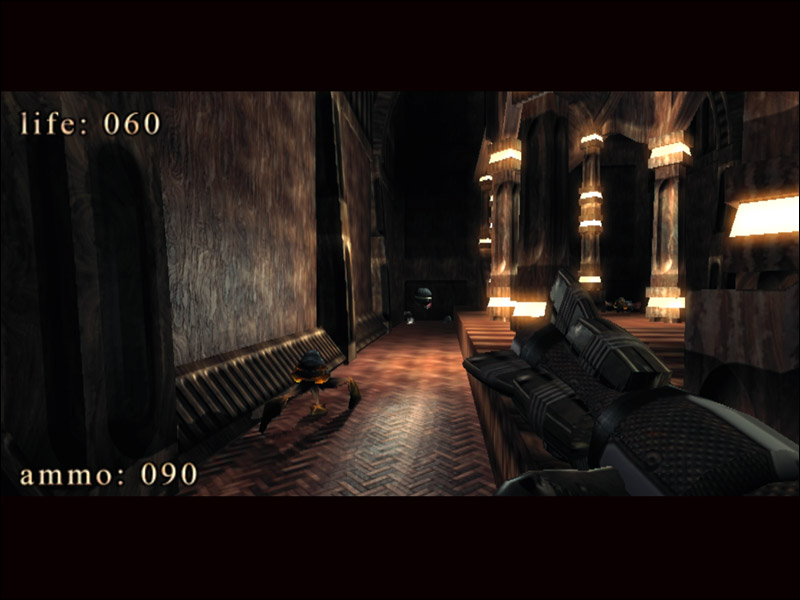
\includegraphics[width=0.5\textwidth]{images/kkrieger}}                
  \subcaptionbox{Doom 3}{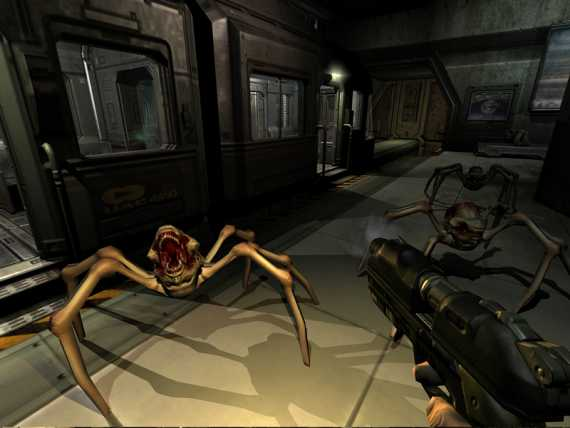
\includegraphics[width=0.5\textwidth]{images/doom3}}                
  \caption{Comparison screenshots of Doom 3 and kkrieger}
  \label{fig:kkriegerdoomcomp}
\end{figure}

\section{Texture Generation}

\subsection{Perlin Noise}
\label{sec:perlinnoise}
Perlin Noise allows us to generate a wide variety of materials based on Ken Perlin's seminal work on the topic in 1985~\cite{Perlin:1985:IS:325165.325247}.
Ken Perlin earned an Academy Award for his invention in 1997~\cite{web:perlinacademy}.
Perlin Noise was first used in Tron to provide some of the textures in the film.
Since then perlin noise has found a lot of applications in many areas such as generating heightmaps for procedurally generated terrain in games and movies.

However, the application which is most important in the context of this project is that it allows for the procedural generation of a wide variety of materials.
Figure~\ref{fig:perlinvase} shows an example vase which is textured using perlin noise.

Perlin noise is seen using a series of semi-random patterns to generate patterns which are suitable for the context.
By experimenting with different values in the algorithm, it is possible to generate a wide variety of materials.
This is shown in Figure~\ref{fig:perlinmaterials}, where 3 very different materials are generated using perlin noise.
Similar techniques are presented in Section~\ref{sec:implPerlin}, where we use perlin noise to generate a variety of materials.

\begin{figure}
  \centering
  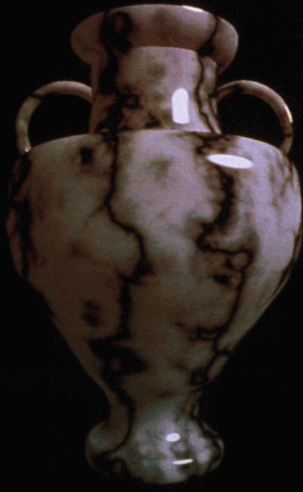
\includegraphics[width=0.4\textwidth]{images/perlinvase}
  \caption{A vase with a texture generated using Perlin Noise. \cite{web:perlinvase}}
  \label{fig:perlinvase}
\end{figure}


\begin{figure}
  \centering
  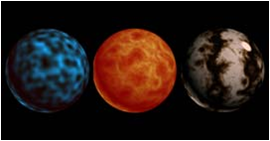
\includegraphics[width=0.5\textwidth]{images/perlinmaterials}
  \caption{Different materials generated using Perlin Noise.}
  \label{fig:perlinmaterials}
\end{figure}


\subsection{Bump Mapping}
\label{sec:bumpmapping}
Bump mapping is a method for simulating the appearance of bumps or wrinkles in an object.
This involves the extracting the normal information for a vertex based on some information, usually an input texture which represents a heightmap.
These new normals are then used in lighting calculations so that the resultant image makes it appear as if there is bumps or wrinkles in the object, even though the geometry itself has not changed.
This is a common technique and is well applied in video games.
Kilgard explained the process in a GDC talk on the topic~\cite{kilgard2000practical}.
There are a few methods but they all involve extracting the normal from an input texture and using this in the lighting calculations.
How the input texture represents the normal and what lighting calculations to use are entirely up to the programmer, based on their needs. 
Kilgard outlines a number of different methods including a new method using multiple textures to generate the required information.

Procedural bump mapping uses a slightly different approach to calculate the normal.
Instead of extracting the normal from an input texture, it is generated based on some mathematical function.
These procedural bump maps are usually calculated directly in the shaders, where they have access to information such as texture coordinates.
Procedural bump maps use some function of this texture coordinate to calculate the normal.

Ebert et. al present a method for procedurally bump mapping a brick-like texture~\cite{ebert2003texturing}.
Figure~\ref{fig:procbricktexture} shows an example of a procedural brick texture generated using their technique.

\begin{figure}
  \centering
  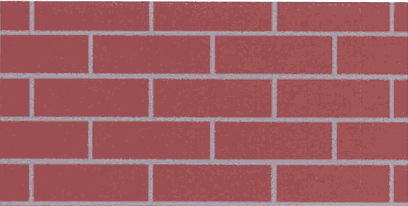
\includegraphics[width=0.4\textwidth]{images/procbricktexture}
  \caption{An example of a procedural normal map to generate a brick texture.}
  \label{fig:procbricktexture}
\end{figure}
